% Don't touch this %%%%%%%%%%%%%%%%%%%%%%%%%%%%%%%%%%%%%%%%%%%
\documentclass[11pt]{article}
\usepackage{fullpage}
\usepackage[left=1in,top=1in,right=1in,bottom=1in,headheight=3ex,headsep=3ex]{geometry}
\usepackage{graphicx}
\usepackage{float}
\usepackage[acronym]{glossaries}

\newcommand{\blankline}{\quad\pagebreak[2]}
%%%%%%%%%%%%%%%%%%%%%%%%%%%%%%%%%%%%%%%%%%%%%%%%%%%%%%%%%%%%%%

\newcommand{\courseCode}{CIT }
\newcommand{\courseTitle}{IOT and Smart City}
\newcommand{\courseType}{TH + PR}
\newcommand{\courseYear}{IV}
\newcommand{\courseSemester}{II}
\newcommand{\courseCreditHour}{2+1=3}
\newcommand{\courseContactHours}{45}
\newcommand{\programName}{Bachelor of Information Technology}
\newcommand{\labHours}{15}
\newcommand{\labType}{Computer Lab}

\newacronym{gis}{GIS}{Geographical Information System}
\newacronym{iot}{IoT}{Internet of Things}
\newacronym{bim}{BIM}{Building Information Modeling}
\newacronym{ai}{AI}{Artificial Intelligence}
\newacronym{ml}{ML}{Machine Learning}

% Modify Course title, instructor name, semester here %%%%%%%%

\title{ \courseTitle}
\author{Gandaki University}
% \date{ \courseYear~Year, \courseSemester~Sem}


%%%%%%%%%%%%%%%%%%%%%%%%%%%%%%%%%%%%%%%%%%%%%%%%%%%%%%%%%%%%%%

% Don't touch this %%%%%%%%%%%%%%%%%%%%%%%%%%%%%%%%%%%%%%%%%%%
\usepackage[sc]{mathpazo}
\linespread{1.05} % Palatino needs more leading (space between lines)
\usepackage[T1]{fontenc}
\usepackage[mmddyyyy]{datetime}% http://ctan.org/pkg/datetime
\usepackage{advdate}% http://ctan.org/pkg/advdate
\newdateformat{syldate}{\twodigit{\THEMONTH}/\twodigit{\THEDAY}}
\newsavebox{\MONDAY}\savebox{\MONDAY}{Mon}% Mon
\newcommand{\week}[1]{%
%  \cleardate{mydate}% Clear date
% \newdate{mydate}{\the\day}{\the\month}{\the\year}% Store date
  \paragraph*{\kern-2ex\quad #1, \syldate{\today} - \AdvanceDate[4]\syldate{\today}:}% Set heading  \quad #1
%  \setbox1=\hbox{\shortdayofweekname{\getdateday{mydate}}{\getdatemonth{mydate}}{\getdateyear{mydate}}}%
  \ifdim\wd1=\wd\MONDAY
    \AdvanceDate[7]
  \else
    \AdvanceDate[7]
  \fi%
}
\usepackage{setspace}
\usepackage{multicol}
%\usepackage{indentfirst}
\usepackage{fancyhdr,lastpage}
\usepackage{url}
\pagestyle{fancy}
\usepackage{hyperref}
\usepackage{lastpage}
\usepackage{amsmath}
\usepackage{layout}


\lhead{}
\chead{}
%%%%%%%%%%%%%%%%%%%%%%%%%%%%%%%%%%%%%%%%%%%%%%%%%%%%%%%%%%%%%%

% Modify header here %%%%%%%%%%%%%%%%%%%%%%%%%%%%%%%%%%%%%%%%%
\rhead{\footnotesize \courseTitle}

%%%%%%%%%%%%%%%%%%%%%%%%%%%%%%%%%%%%%%%%%%%%%%%%%%%%%%%%%%%%%%
% Don't touch this %%%%%%%%%%%%%%%%%%%%%%%%%%%%%%%%%%%%%%%%%%%
\lfoot{}
\cfoot{\small \thepage/\pageref*{LastPage}}
\rfoot{}

\usepackage{array, xcolor}
\usepackage{color,hyperref}
\definecolor{clemsonorange}{HTML}{EA6A20}
\hypersetup{colorlinks,breaklinks,linkcolor=clemsonorange,urlcolor=clemsonorange,anchorcolor=clemsonorange,citecolor=black}

\begin{document}

\maketitle

\blankline

\begin{tabular*}{.93\textwidth}{@{\extracolsep{\fill}}lr}

%%%%%%%%%%%%%%%%%%%%%%%%%%%%%%%%%%%%%%%%%%%%%%%%%%%%%%%%%%%%%%

% Modify information %%%%%%%%%%%%%%%%%%%%%%%%%%%%%%%%%%%%%%%%%
Program: \texttt{\programName} & \\
Subject: \texttt{\courseTitle} %& Year: \courseYear  \\

% Course Code: {\courseCode} &  Semester: \courseSemester \\

%  Credit Hour: \courseCreditHour & Lab Type: \labType \\
% %  & \\
%  Contact Hours: \courseContactHours & Lab Hours: \labHours \\
&  \\
\hline
\end{tabular*}

\vspace{5 mm}

% Starting Section %%%%%%%%%%%%%%%%%%%%%%%%%%%%%%%%%%%%%%%%%%%%


\section{Course Objectives}
The key objectives of learning \courseTitle are:
\begin{enumerate}
  \item Learn and understand how various technologies work together in DevOps. Get a firm understanding in DevOps Processess, Tools and Technologies.
  
  \item Learn the basics of working in DevOps environments like Linux, AWS, Bash \& Python Scripting, Jenkins, Ansible, Docker, Kubernetes and more
  
  
\end{enumerate}

% First Section %%%%%%%%%%%%%%%%%%%%%%%%%%%%%%%%%%%%%%%%%%%%


\section*{Course Description}


% SEO stands for Search Engine Optimization. SEO is the process of improving the quality and quantity of website traffic to a website and a web page's ranking on search engines such as Google and Bing.

\bigskip
This course will prepare students for a successful career with a comprehensive take on digital marketing and a strong emphasis on the application of theory to practice, in subject areas such as online advertising, social media, content marketing, analytics, consumer psychology and digital advertising. It has been designed for students who are interested in fields such as marketing, media, management and social sciences.


\bigskip
This course will also help you to gain knowledge on how to complete a competitive analysis on a webpage, develop a solid approach for achieving a productive and successful relationship with your client, create influencer relationships and collaborations and analyze data to see which content gets the most shares, create a final report of your findings and recommendations for SEO and present your recommendations to your client. The practical SEO training part of the course shows you how to increase traffic to your website and improve your conversion rate. 

\bigskip
Digital Marketing is the advertising, networking or positioning of a brand, marketing of products and services online through technology. In essence, digital marketing refers to all online activities such as websites, social media and search engine optimization.

% Second Section %%%%%%%%%%%%%%%%%%%%%%%%%%%%%%%%%%%%%%%%%%%

\section{Course Outcomes}

\begin{itemize}
\item This course will enable students to gain hands-on experience in various technical areas, such as programming languages, database management, networking, and cybersecurity.
\item This course will enable students to develop a deeper understanding of the IT industry in Nepal, including its trends, challenges, and opportunities.
\item The program will help students to develop critical thinking and problem-solving skills by working on real-world IT projects and addressing technical issues faced by the organization.
\item The program will enable students to enhance collaboration and project management skills by working closely with IT professionals and participating in team projects, fostering effective communication and teamwork.
\item The students will gain practical experience and skills that enhance employability in the IT industry, preparing for future career opportunities in Nepal's IT sector

\end{itemize}

% Third Section %%%%%%%%%%%%%%%%%%%%%%%%%%%%%%%%%%%%%%%%%%%
% 
\section{Prerequisites/Corequisites}
Prerequisites: MA 116, ... .  Corequisites: ... .

% Fourth Section %%%%%%%%%%%%%%%%%%%%%%%%%%%%%%%%%%%%%%%%%%%
\section{Course Content}

\subsection{Overview of \acrfull{iot} \hfill { 4 Hrs.}}

\begin{enumerate}
    \item Definition of \acrfull*{iot}
    \item Trends of \acrshort*{iot}: History and Growth of the \acrshort*{iot} industry. Industries being powered by \acrshort{iot}.
    \item Fundamental components of \acrshort{iot} system
    \item Applications of \acrshort{iot}
\end{enumerate}

\subsection{Sensors and Devices used in \acrshort*{iot} \hfill {6 Hrs.}}

\begin{enumerate}
    \item Overview of Sensors and Devices.
    \item \acrfull*{iot} Device Hardware
    \item Scaling, Manufacturing and Shipping.
    \item Gateways
    
\end{enumerate}

\subsection{Connectivity \hfill {4 Hrs.}}

\begin{enumerate}
    \item Introduction to Connectivity.
    \item Cellular connectivity for \acrshort{iot}.
    \item Satellite connectivity for \acrshort{iot}.
    \item WiFi/Bluetooth/LPWAN connectivity for \acrshort{iot}.
    
\end{enumerate}

\subsection{Data Processing \hfill {4 Hrs.}}
\begin{enumerate}
    \item Introduction to the Cloud.
    \item Introduction to \acrfull{iot} Platform.
    \begin{itemize}
        \item Organization Strategies to choose an \acrshort{iot} platform.
        \item Types of \acrfull{iot} Platform
        \item Needs to migrate to an \acrfull{iot} Platform.
    \end{itemize}
    \item EDGE Computing and FOG Computing
    \item APIs to integrate \acrshort{iot} to custom application.
    
\end{enumerate}

\subsection{\acrshort{iot} Protocols and Machine Learning \hfill {9 Hrs.}}
\begin{enumerate}
    \item Overview of \acrshort{iot} Protocols.
    \item \acrfull{iot} Protocols: Data Protocols 
    \begin{itemize}
        \item MQTT
        \item CoAP
        \item AMQP
        \item M2M Communication Protocol
        \item XMPP
    \end{itemize}
    \item \acrfull{iot} Protocols: Network Protocols 
    \begin{itemize}
        \item HTTP
        \item LoRaWAN
        \item Bluetooth
        \item ZigBee
    \end{itemize}
    \item Machine Learning for \acrshort{iot}
\end{enumerate}

\subsection{User Interface and User Experience in \acrshort{iot} \hfill{2 Hrs.}}
\begin{enumerate}
    \item Introduction to UI/UX for \acrshort{iot}
    \item Key considerations for UI/UX.
    \item Recent trends in designing UI/UX for \acrshort{iot}.
\end{enumerate}

\subsection{Security and Privacy in \acrshort*{iot} \hfill{4 Hrs.}}
\begin{enumerate}
    \item IoT security challenges and threats
    \item Authentication and access control in IoT systems
    \item Data privacy and compliance in smart cities
    \item Security best practices for IoT deployments
\end{enumerate}

\subsection{\acrshort{iot} for Smart Cities \hfill{3 Hrs.}}
\begin{enumerate}
    \item Introduction to smart city.
    \item Needs for smart cities transformation.
    \item Roles of \acrfull{iot} in Smart Cities.
    \item Case Studies of Smart City.
\end{enumerate}

\subsection{Other technologies in Smart City \hfill {3 Hrs.}}
\begin{enumerate}
    \item \acrfull{bim} and \acrfull{gis} value for smart cities.
    \begin{itemize}
        \item BIM Dimensions
        \item Sustainability and Facility Management in BIM
        \item BIM Lifecycle
        \item Integrating BIM and GIS
    \end{itemize}
    \item Big Data
    \item Case Study: Applications of Smart City.
\end{enumerate}

\subsection{Smart City Design \hfill{6 Hrs.}}
\begin{enumerate}
    \item Smart energy management and grid systems
    \item Smart transportation and traffic management
    \item Environmental monitoring and sustainability
    \item Smart buildings and infrastructure
    \item Citizen participation in smart city initiatives
\end{enumerate}

% Fifth Section %%%%%%%%%%%%%%%%%%%%%%%%%%%%%%%%%%%%%%%%%%%

% \subsection{Assessments}

% ...

\section{Case Study}
\begin{enumerate}
    \item  Study on different search engines like Google, Bing etc and key business strategies incorporated by those engines.
    \item Study of different web development frameworks for SEO.
    \item A case study of SEO and digital marketing in a business(choosen by student) domain: Global and Local Perspective.
\end{enumerate}

% Sixth Section %%%%%%%%%%%%%%%%%%%%%%%%%%%%%%%%%%%%%%%%%%%
% \subsubsection{Lab}
% \begin{enumerate}
%     \item 
% \end{enumerate}

\section{Laboratory Work}

\subsection{Lab Contents}
\begin{enumerate}
    \item \textbf{Introduction to IoT Development Platforms} (3 Hrs.)
    \begin{itemize}
        \item Setting up Raspberry Pi/Arduino
        \item Basic Programming for IoT Devices
    \end{itemize}
    \item \textbf{Sensors and Actuators} (4 Hrs.)
    \begin{itemize}
        \item Connecting and Programming Sensors
        \item Real-world Application Development
    \end{itemize}
    \item \textbf{IoT Communication} (4 Hrs.)
    \begin{itemize}
        \item Network Setup for IoT Devices
        \item Data Transmission and Reception
    \end{itemize}
    \item \textbf{Data Collection and Processing} (4 Hrs.)
    \begin{itemize}
        \item Data Collection from Sensors
        \item Basic Data Processing and Visualization
    \end{itemize}
    \item \textbf{IoT Project Development} (4 Hrs.)
    \begin{itemize}
        \item Project Planning and Development
        \item Presentation and Demonstration
    \end{itemize}
\end{enumerate}


% Reference Books Section


\section{TextBooks}
\begin{enumerate}
    \item Internet of Things: A Hands-On Approach, Arshadeep Bahga, Vijay Madisetti, 2014.
    \item Introduction to IoT, Cambridge University Press, Sudip Mishra, Anandarup Mukherjee, Arijit Roy, 2021.
\end{enumerate}

\section{Reference Books}
\begin{enumerate}
    \item The Internet of Things: From Data to Insight, John Davies, Carolina Fortuna, 2020.
    \item IoT and Cloud Computing for Societal Good, Jitendra Kumar Verma, Deepak Saxena, Vicente González-Prida, 2021.
    \item 5G and Beyond: The Future of IoT, Parag Chatterjee, Robin Singh Bhadoria, Yadunath Pathak, 2022.
\end{enumerate}

% Appendix Section %%%%%%%%%%%%%%%%%%%%%%%%%%%%%%%%%%%%%%%%%%%
% \subsection*{Grading Policy}
The typical NC State grading scale will be used. I reserve the right to curve the scale dependent on overall class scores at the end of the semester. Any curve will only ever make it easier to obtain a certain letter grade. The grade will count the assessments using the following proportions:
\begin{itemize}
	\item \underline{\textbf{30\%}} of your grade will be determined by 2 in class midterm exams (15\% each).
	\item \underline{\textbf{5\%}} of your grade will be determined by ...
	\item \underline{\textbf{5\%}} ...
    \item \underline{\textbf{10\%}}  ...
	\item \underline{\textbf{15\%}} ...
	\item \underline{\textbf{15\%}} ...
\end{itemize}

% Add a figure %%%%%%%%%%%%%%%%%%%%%%%%%%%%%%%%%%%%%%%%%%%

% \begin{figure*}
% 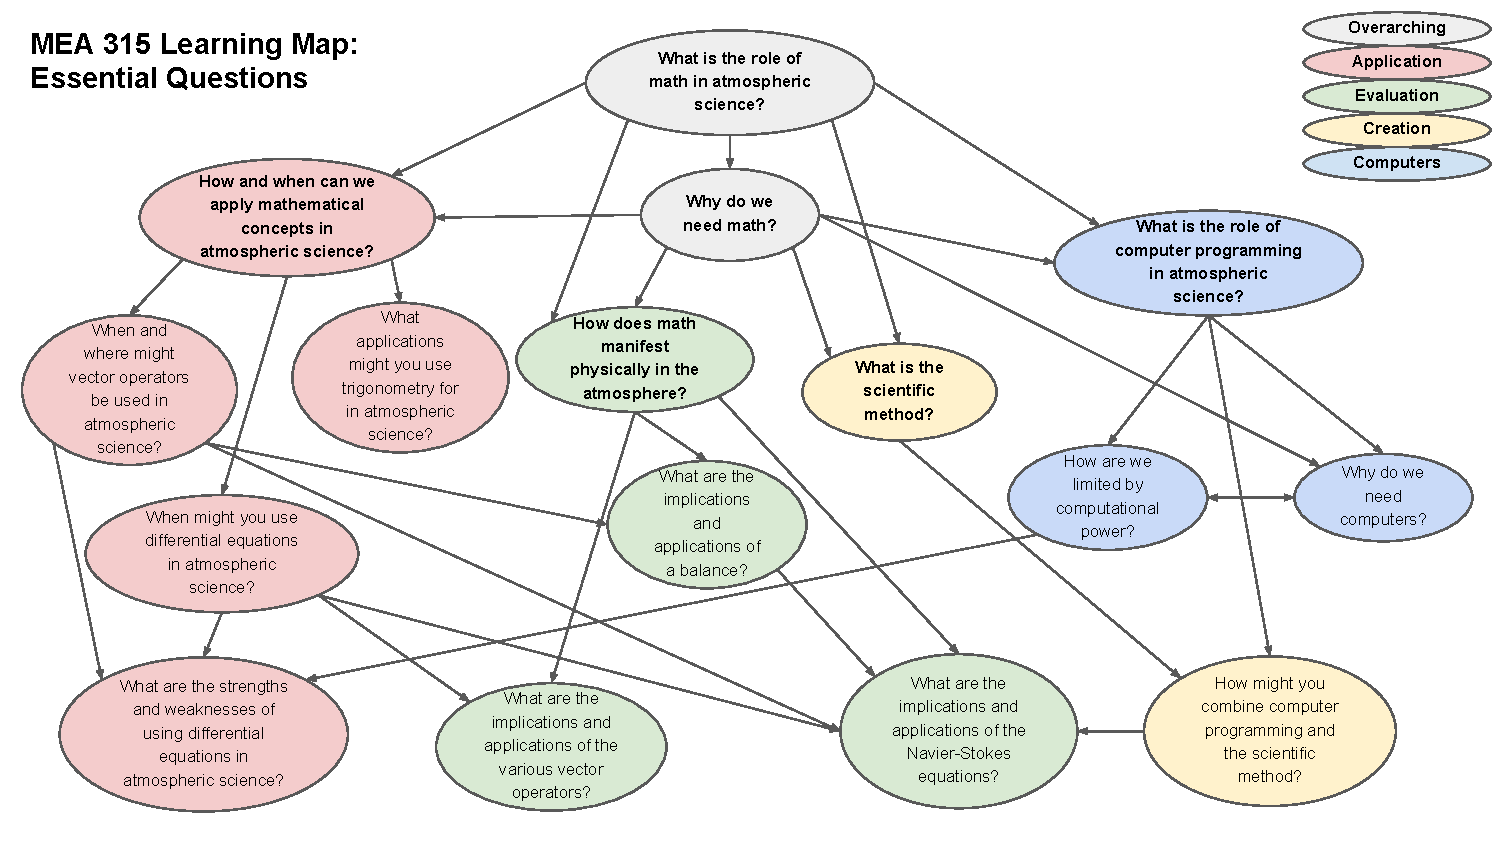
\includegraphics[width=1.3\textwidth,angle=90]{Concept_map_315.pdf}
% \end{figure*}

% Fifth Section %%%%%%%%%%%%%%%%%%%%%%%%%%%%%%%%%%%%%%%%%%%

\newpage
\section*{Course Policies}

\subsection*{During Class}
\footnotesize{I understand that the electronic recording of notes will be important for class and so computers will be allowed in class. Please refrain from using computers for anything but activities related to the class. Phones are prohibited as they are rarely useful for anything in the course. Eating and drinking are allowed in class but please refrain from it affecting the course. Try not to eat your lunch in class as the classes are typically active.}

\subsection*{Attendance Policy}
\footnotesize{For complete attendance and excused absence policies, please see http://policies.ncsu.edu/regulation/reg-02-20-03. Attendance is expected in all lecture and lab sections. Valid excuses for absence will be accepted before class. In extenuating circumstances, valid excuses with proof will be accepted after class. For every class missed the participation grade will be dropped 1 point.}

\subsection*{Policies on Incomplete Grades and Late Assignments}
\footnotesize{If an extended deadline is not authorized by the instructor or department, an unfinished incomplete grade will automatically change to an F after either (a) the end of the next regular semester in which the student is enrolled (not including summer sessions), or (b) the end of 12 months if the student is not enrolled, whichever is shorter. Incompletes that change to F will count as an attempted course on transcripts. The burden of fulfilling an incomplete grade is the responsibility of the student. The university policy on incomplete grades is located at http://policies.ncsu.edu/regulation/reg-02-50-3.}

\footnotesize{Late assignments will be accepted for no penalty if a valid excuse is communicated to the instructor before the deadline. After the deadline, assignments will be accepted for a 50\% deduction to the score up to 2 days after the deadline. After this any assignments handed in will be given 0.}

\subsection*{Academic Integrity and Honesty}
\footnotesize{Students are required to comply with the university policy on academic integrity found in the Code of Student Conduct found at http://policies.ncsu.edu/policy/pol-11-35-01. Don't cheat. Don't be that guy. Yes, you. You know exactly what I'm talking about. See http://policies.ncsu.edu/policy/pol-11-35-01 for a detailed explanation of academic honesty.}

\subsection*{Accommodations for Disabilities}
\footnotesize{Reasonable accommodations will be made for students with verifiable disabilities. In order to take advantage of available accommodations, students must register with the Disability Services Office at Suite 2221, Student Health Center, Campus Box 7509, 919-515-7653. For more information on NC State's policy on working with students with disabilities, please see the Academic Accommodations for Students with Disabilities Regulation (REG02.20.01) (https://policies.ncsu.edu/regulation/reg-02-20-01/).
Non-Discrimination Policy NC State University provides equality of opportunity in education and employment for all students and employees. Accordingly, NC State affirms its commitment to maintain a work environment for all employees and an academic environment for all students that is free from all forms of discrimination.}

\footnotesize{Discrimination based on race, color, religion, creed, sex, national origin, age, disability, veteran status, or sexual orientation is a violation of state and federal law and/or NC State University policy and will not be tolerated. Harassment of any person (either in the form of quid pro quo or creation of a hostile environment) based on race, color, religion, creed, sex, national origin, age, disability, veteran status, or sexual orientation also is a violation of state and federal law and/or NC State University policy and will not be tolerated. Retaliation against any person who complains about discrimination is also prohibited. NC State's policies and regulations covering discrimination, harassment, and retaliation may be accessed at \href{http://policies.ncsu.edu/policy/pol-04-25-05} or  \href{http://www.ncsu.edu/equal_op/}. Any person who feels that he or she has been the subject of prohibited discrimination, harassment, or retaliation should contact the Office for Equal Opportunity (OEO) at 919-515-3148.}

% 
% Course Schedule %%%%%%%%%%%%%%%%%%%%%%%%%%%%%%%%%%%%%%%%%%%

\newpage
\section*{Schedule and weekly learning goals}

The schedule is tentative and subject to change. The learning goals below should be viewed as the key concepts you should grasp after each week, and also as a study guide before each exam, and at the end of the semester. Each exam will test on the material that was taught up until 1 week prior to the exam (i.e. vorticity will not be tested until exam 2). The applications in the second half of the semester tend to build on the concepts in the first half of the semester though, so it is still important to at least review those concepts throughout the semester.

% Set first date of the semester (for some reason this is a week before what comes up, but that's easy to get around)
\SetDate[01/01/2018]
\week{Week 01} Topic 1
\begin{itemize}
\item Goal 1
\item Goal 2
\item Goal 3
\end{itemize}

\week{Week 02} Topic 2
\begin{itemize}
\item Goals ...
\end{itemize}

\week{Week 03} Topic 3
\begin{itemize}
\item Goals ...
\end{itemize}

\week{Week 04} ...
\begin{itemize}
\item 
\end{itemize}

\week{Week 05} ...
\begin{itemize}
\item 
\end{itemize}

\week{Week 06} ...
\begin{itemize}
\item 
\end{itemize}

\week{Week 07} ...
\begin{itemize}
\item 
\end{itemize}

\week{Week 08} ... and \textbf{Exam 1}
\begin{itemize}
\item 
\end{itemize}

\week{Week 09} Spring Break

\week{Week 10} ...
\begin{itemize}
\item 
\end{itemize}

\week{Week 11} ...
\begin{itemize}
\item ...
\end{itemize}

\week{Week 12} ...
\begin{itemize}
\item ...
\end{itemize}

\week{Week 13} ...
\begin{itemize}
\item ...
\end{itemize}

\week{Week 14} ...
\begin{itemize}
\item ...
\end{itemize}

\week{Week 15} ... and  \textbf{Exam 2}

\week{Week 16} ...

\week{Week 17} \textbf{Final Exam}





\end{document}